\documentclass[11pt]{IEEEtran}
\usepackage[brazilian]{babel}
\usepackage[utf8]{inputenc}
\usepackage[T1]{fontenc}
\usepackage{float}
\usepackage{graphicx}
\usepackage{caption}

\captionsetup[table]{skip=10pt}

\sloppy

\title{Programação Paralela\\ Trabalho II}

\author{Giovanni Cupertino, Matthias Nunes, \IEEEmembership{Usuário pp12820}}

\begin{document}

\maketitle

\section{Introdução}

O objetivo do trabalho é desenvolver uma solução que ordene um vetores, em casos de teste diferentes, utilizando o algoritmo do bubble sort. Os vetores utilizados possuem dois tamanhos que são de cem mil elementos e outro com um milhão que estão na ordem inversa de valores. 
Para abordagem paralela do trabalho, utilizou-se o modelo de divisão e conquista criando uma estrutura de árvore binária. Para esta abordagem cada nó da árvore decide se vai ser dividido ou conquistado por meio de um valor fixo denominado delta, no qual, caso o vetor seja maior que o delta, o processo divide o vetor para seus dois filhos, em partes iguais, e os seus filhos repetem o processo até que o vetor seja menor ou igual ao delta, optando assim por conquista-lo. Para conquistar o processo executa o algoritmo de ordenação e depois devolve o pedaço do vetor já ordenado para o seu pai que terá de fazer o método de intercalação- que consiste em juntar vetores ordenados e gerar um novo também ordenado- com os dois vetores que irá receber e repetir o processo a raiz onde se terá o valor ordenado, após a intercalação.
Para otimizar o algoritmo, que tem o trabalho de ordenação somente nas folhas da árvore, e para não manter os processos, que não são folhas, esperando foi criada uma versão otimizada que consiste em ter a ordenação de parte do trabalho no processo local e a outra parte ser passada dividida para os dois filhos diminuindo o tempo que os processos ficam em espera.   



\section{Análise dos Resultados Obtidos}

A analise dos dados foi feita baseada no pior caso ,do problema apresentado, que é o vetor de um milhão de posições. Para o caso do vetor de cem mil posições também foram coletados os tempos e podem ser observados na tabela. 
Em primeirá analise é possível observar que no caso sem otimização o tempo de resposta diminui e o speed-up aumentou, ultrapassando até mesmo o speed-up ideal com o aumento do número de processos, isso ocorre devido não só ao fato de ter mais processos em execução mas também pelo algoritmo de ordenação possuir uma notação O(n²) que permite a cada divisão no vetor uma melhora quadratica no tempo para a ordenação da nova parte. É possível observar também que a eficiência também aumenta com o aumento do número de processos em execução, entretanto de 15 para 31 threads a eficiência diminui um pouco já que devido a estrutura ser de uma árvore binária o número de vezes que o método de intercalação vai precisar ser executado e a quantidade de mensagens enviadas vai aumentando bastante por altura da árvore o que reduz um pouco o benefício ganho com a divisão. Outra questão e que devido ao trabalho de ordenação estar somente nas folhas, neste caso, é necessário eles esperar toda a ordenação por elas para depois realizar as intercalações necessárias o que pode deixar os processos esperando por bastante tempo sem realizar nenhuma tarefa.
Observando que ao executar em paralelo, sem otimizar, vários processos ficavam esperando para realizar uma tarefa, a versão otimizada tem como modo de resolução para este problema ter uma parte do vetor para ordenar localmente e realizar a divisão do resto dele para para seus dois filhos(mesma quantidade para cada um e caso sobre um pouco ele ordena esta parte) até um ponto em que o vetor passado é menor ou igual ao delta. Para determinar o delta, que é a quantidade do vetor que será ordenado localmente para o caso otimizado, utilizamos o tamanho do vetor original dividido pelo número de processos, depois de pegar sua parte o nodo pai distribui igualmente o resto da tarefa. Com isso foi possível obter resultados muito melhores do que o algoritmo sem otimização visto que ele começa a distribuir parte menores de trabalhos nas divisões e utiliza o tempo que os outros processos  demoram para realizar a sua ordenação local, mesmo ainda existindo uma perda de tempo pelas trocas de mensagens e para o método de intercalação.
O fato de se estar utilizando a biblioteca MPI\@ e dois nós da maquina atlantica permitiu um balanceamento da carga entre os núcleos e threads destes nós e há uma possível perda nos tempos de resposta para a comunicação que não teve relevância para a análise realizada. A utilização de mais de 16 processos(hyper-threading, já que passa da soma dos núcleos dos dois nós) apresentou uma melhoria significativa nos tempos de resposta e no speed-up devido a permitir dividir o problema em mais pedaços e tirar proveito do algoritmo de ordenação. A utilização de outro algoritmo de ordenação mais rápido permitiria um tempo de execução menor mas não seria observado tamanha diferença entre seus valores para diferentes números de processos como foi possível observar com o bubble sort.


	\begin{table}[H]
		\centering
		%\scalebox{0.8}{
			\begin{tabular}{c|r|r|r|r}
				Processos & Normal & Otimizado & Normal O3 & Otimizado O3 \\
				\hline
				3  & 11,197245s & 5,030874s & 2,494979s & 1,122686s \\
				\hline
				7  &  2,864694s & 0,924965s & 0,639917s & 0,221029s \\
				\hline
				15 &  0,911735s & 0,360175s & 0,229385s & 0,080532s \\
				\hline
				31 &  0,379110s & 0,115022s & 0,077629s & 0,042855s \\
			\end{tabular}
		%}
		\caption{Resultados obtidos para 100000}
		\label{result_table}
	\end{table}

	\begin{table}[H]
		\centering
		%\scalebox{0.8}{
			\begin{tabular}{c|r|r|r|r}
				Processos & Normal & Otimizado & Normal O3 & Otimizado O3 \\
				\hline
				3  & 1118,725370s & 504,497851s & 260,702105s & 116,810162s \\
				\hline
				7  &  283,095140s &  92,283123s &  65,604866s & 21,520253s \\
				\hline
				15 &   73,926856s &  21,100409s &  16,904703s & 4,794249s \\
				\hline
				31 &   36,979798s &   9,868190s &   6,390105s & 1,807969s \\
			\end{tabular}
		%}
		\caption{Resultados obtidos para 1000000}
		\label{result_table}
	\end{table}

	%\begin{figure}[H]
		%\centering
		%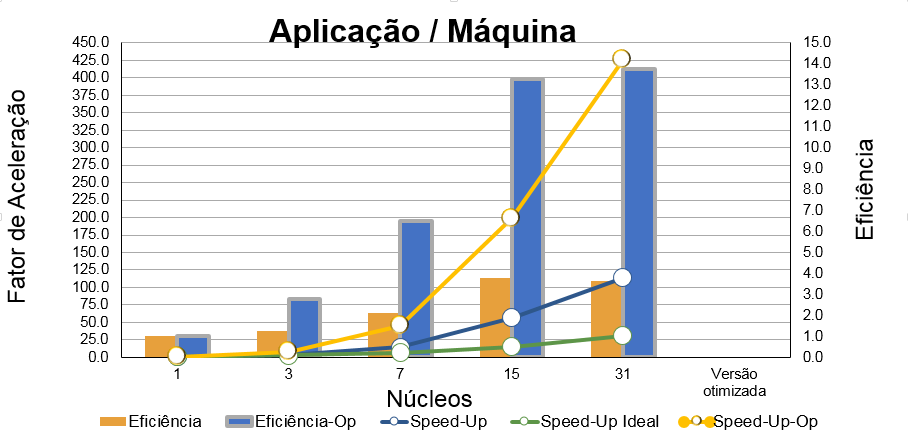
\includegraphics[width=88mm]{doc/graph.png}
		%\caption{Gráfico gerado a partir da tabela}
		%\label{fig_graph}
	%\end{figure}

\section{Dificuldades Encontradas}

	Não foram encontradas dificuldades na implementação desse trabalho, nem na
	utilização da biblioteca MPI\@.

\end{document}

